\documentclass{ctexart}
\usepackage{listings}
\usepackage{graphicx}
\usepackage{geometry}
\usepackage{float}
\usepackage[colorlinks=true,linkcolor=black]{hyperref}
\usepackage[format=hang,font=small,textfont=it]{caption}
\usepackage[nottoc]{tocbibind}
\usepackage{fontspec}
\usepackage{xeCJK}
\setCJKmainfont{楷体}
\geometry{a4paper,centering,scale=0.8}

\begin{document}

\title{\heiti C++程序设计---宠物小精灵实验报告}
\author{学号-2014211281-黄智伟}
\date{\today}

\maketitle
\tableofcontents

\pagebreak[4]

\section{设计任务的描述}
\label{sec:purpose}
应用面向对象的设计方法来设计一款平台类对战游戏。

\section{运行环境}
\label{sec:environment}
\begin{enumerate}
  \item 系统:kali
  \item 编程环境:qt5.7
  \item 数据库:mysql
\end{enumerate}

\section{功能需求说明}
\label{sec:demand}
\subsection{第一阶段}
实现小精灵类的设计,包括小精灵种类,各种属性及攻击方式设计,同时编写测试函数进行是测试。
\subsection{第二阶段}
\begin{enumerate}
  \item 每个用户需要注册一个账号,用户名全局唯一,不能有任何两个用户名相同,要考虑注册失败的场景时的反馈。
  \item 实现注册、登录、登出功能,均采用C/S模式,客户端和服务端用socket进行通信,服务端保存所有用户的信息。
  \item 每个用户拥有:用户名、拥有的精灵,两个属性。 用户注册成功时,系统自动随机分发三个1级精灵给用户。
  \item 用户可以查看所有成功注册用户拥有的精灵,也可以查看所有当前在线的用户。
\end{enumerate}
\subsection{第三阶段}
\begin{enumerate}
  \item 实现用户小精灵与系统进行升级赛,升级可获得经验,进而升级。
  \item 实现用户小精灵与系统进行决斗赛,战胜可获得此精灵,战败则系统从用户的精灵中随机选三个(不够三个精灵的情况就选择他所有的精灵),然后由用户选一个送出。
  \item 用户如果没有精灵(比如总是失败,已经全部送出去),则系统会随机放给给他一个初级精灵。
  \item 实现用户可查看某一用户胜率的功能。
  \item 用户增加新属性:宠物个数徽章(金银铜)和高级宠物徽章(金银铜),分别根据拥有的宠物个数的多少和拥有高级宠物(15级)个数的多少颁发。
\end{enumerate}

\section{具体实现}
\label{sec:realization}
\subsection{第一阶段}
\subsubsection{基类设计}
主要数据类型:
\lstset{language=C++}
\begin{lstlisting}
  enum KIND//四种类型
  {
      HIGH_ATTACK,HIGH_BLOOD,HIGH_DEFENSE,HIGH_SPEED
  };
  const QList<QString> POKEMONNAME={
      "Feraligatr",//大力鳄
      "Charizard",//喷火龙
      "Noivern",//音波龙
      "Bagon",//宝贝龙
      "Glaceon",//冰伊布
      "Pikachu",//皮卡丘
      "Wynaut",//小果然
      "Doduo",//嘟嘟
  };//pokemon名字

  enum SKILL//技能
  {
      HydroCannon,//加农水炮
      Cut,//居合斩
      LeechLife,//吸血
      FocusEnergy,//聚气
      Barrier,//屏障
      LightScreen,//光墙
      Counter,//双倍奉还
      TriAttack,//三重攻击
      NormalAttack,//普通攻击
  };

  enum QUALIFICATION{
      S,SS,SSS
  };//属性等级

  class Pokemon : public QObject
  {
      Q_OBJECT
  public:
      Pokemon():level(1),experience(0){}
      virtual ~Pokemon(){}

      virtual uint Attack(){return 0;}//精灵技能
      void ExperienceUp(uint value);
      virtual void LevelUP(){}

      QString getName();
      uint getLevel();
      QString getInformation();
  protected:
      QString name;     //名字
      uint level;       //等级
      uint experience;  //经验
      uint attack;      //攻击属性
      uint blood;       //生命属性
      uint currentBlood;//实时血量,对决时使用
      uint defense;     //防御属性
      uint speed;       //敏捷属性
      uint kind;        //种类
      uint attr;        //稀有度
      SKILL skill;       //技能

      void setValues(uint baseAttack, uint baseBlood, uint baseDefense,
                     uint baseSpeed);

  signals:

  public slots:
  };
\end{lstlisting}
\ \ \ 主要函数:
\lstset{language=C++}
\begin{lstlisting}
  void Pokemon::ExperienceUp(uint value)//增加经验函数

  QString Pokemon::getName()//小精灵名字的get函数

  uint Pokemon::getLevel()//小精灵等级的get函数

  QString Pokemon::getInformation()//小精灵各种属性的get函数

  void Pokemon::setValues(uint baseAttack, uint baseBlood, uint baseDefense,
                          uint baseSpeed)//小精灵各种属性的set函数
\end{lstlisting}
\subsubsection{子类实现}
以HighAttack子类为例:
\lstset{language=C++}
\begin{lstlisting}
    uint HighAttack::Attack()//攻击函数
    {
        qsrand (QTime::currentTime ().msec ());
        uint probability=qrand ()%10;
        if(probability<8)//普通攻击
            return NormalAttack;
        else             //20%几率使用技能
            return this->skill;
    }

    void HighAttack::LevelUP()//升级函数
    {
        this->level++;

        this->attack+=100;
        this->blood+=50;
        this->currentBlood=this->blood;//升级后当前的血量回复满血
        this->defense+=50;
        this->speed+=50;
    }
\end{lstlisting}

\subsection{第二阶段}
\subsubsection{数据结构}
\label{sec:datastruct}
\begin{enumerate}
  \item UDP数据包类型:
  \lstset{language=C++}
  \begin{lstlisting}
    const uint SIGNUP=1;
    const uint SIGNIN=2;
    const uint NAMEEXIST=3;
    const uint SIGNUPOK=4;
    const uint NOSUCHUSER=5;
    const uint PWDDIFF=6;
    const uint SIGNINOK=7;
    const uint PKMDATA=8;
    const uint SIGNOUT=9;
    const uint ONLINEUSERS=10;
    const uint ALLUSERS=11;
  \end{lstlisting}
  \item mysql中的users表(第二阶段只使用列username和password,列win和lose为第三阶段使用):
  \begin{figure}[H]
    \centering
    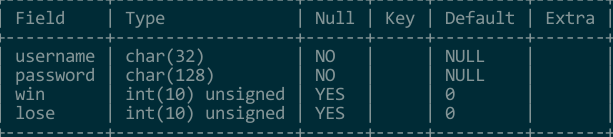
\includegraphics[width=15cm]{users.png}
  \end{figure}
  \item mysql中的pokemon表:
  \begin{figure}[H]
    \centering
    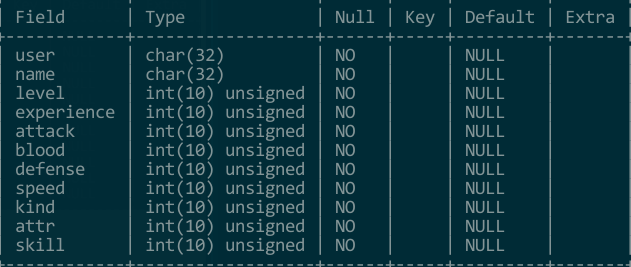
\includegraphics[width=15cm]{pokemon.png}
  \end{figure}
  \item 在线用户类(用于发送在线用户数据时的序列化):
  \lstset{language=C++}
  \begin{lstlisting}
    struct User//在线用户
    {
        QString username;//用户名
        uint port;//端口号

        bool operator==(const User &user) const
        {
            return this->username==user.username&&this->port==user.port;
        }

        //友元声明,一对用于支持QDataStream 输入输出的函数
        friend QDataStream &operator<<(QDataStream &stream, const User &user);
        friend QDataStream &operator>>(QDataStream &stream, User &user);
    };
  \end{lstlisting}
  \item 所有用户数据类(用于发送所有用户数据时的序列化):
  \lstset{language=C++}
  \begin{lstlisting}
    struct UserData
    {
        QString username;//用户名
        QList<UDPPkm*> pkm;//小精灵

        ~UserData()
        {
            for(int i=0;i<3;i++)
                delete this->pkm[i];
        }

        //友元声明,一对用于支持QDataStream 输入输出的函数
        friend QDataStream &operator<<(QDataStream &stream,
                                       const UserData &userData);
        friend QDataStream &operator>>(QDataStream &stream, UserData &userData);
    };
  \end{lstlisting}
  \item pokemon数据包类(小精灵的数据):
  \lstset{language=C++}
  \begin{lstlisting}
    struct UDPPkm
    {
        QString name;     //名字
        uint level;       //等级
        uint experience;  //经验
        uint attack;      //攻击属性
        uint blood;       //生命属性
        uint currentBlood;//实时血量,对决时使用
        uint defense;     //防御属性
        uint speed;       //敏捷属性
        uint kind;        //种类
        uint attr;        //稀有度
        uint skill;       //技能

        //友元声明,一对用于支持QDataStream 输入输出的函数
        friend QDataStream &operator<<(QDataStream &stream, const UDPPkm &pkm);
        friend QDataStream &operator>>(QDataStream &stream, UDPPkm &pkm);
    };
  \end{lstlisting}
\end{enumerate}
\subsubsection{服务器端实现}
服务器监听6665端口,一有数据到达就调用readPendingDatagrams()函数分析客户端请求的种类并调用相应的
函数处理。在线用户由服务器端用一个列表实现,用户注册及登录时将该用户加入列表中,登出从列表中移除。
\begin{enumerate}
  \item 系统随机生成三个小精灵给用户\\
    void CreatePkm(QString user);//随机分配小精灵
  \item 将生成的小精灵存入数据库\\
    void PutIntoSql(QString user, UDPPkm *pkm);
  \item 发送小精灵数据\\
    void SentPkm(QDataStream \&dsOut, QString user);//发送小精灵的数据
  \item 发送在线用户给客户端\\
    void SentOnlineUsers(uint port);//发送在线用户
  \item 发送所有用户数据给客户端\\
    void SentAllUsers(uint port);//发送注册用户
  \item 分析客户端请求并处理
  \lstset{language=C++}
  \begin{lstlisting}
    void MainWindow::readPendingDatagrams()
    {
      ...
      if(loginKind==SIGNUP)
      {
          判断用户是否已存在,并进行处理,返回结果给请求的客户端
      }
      else if(loginKind==SIGNIN)
      {
          验证该用户是否存在及密码正确与否,进行处理,并返回结果给请求的客户端
      }
      else if(loginKind==SIGNOUT)
      {
          用户登出,清楚服务器端的在线用户列表
      }
      else if(loginKind==ONLINEUSERS)
      {
          发送在线用户给客户端
      }
      else if(loginKind==ALLUSERS)
      {
          发送所有用户给客户端
      }
    }
  \end{lstlisting}
\end{enumerate}
\subsubsection{客户端实现}
客户端提供与用户交互的界面,并接受用户的输入,显示服务器返回的数据。客户端分为两个界面,一个为登录注册界面,
另一个为主界面,显示小精灵数据,并提供用户查询在线用户及所有用户的操作界面。启动客户端时检查默认端口(6666)
是否已被占用,若是则端口号加一。
\begin{enumerate}
  \item 登出\\
    void on\_BtnLoginOut\_clicked();
  \item 查询在线用户(发送UDP数据包查询)\\
    void on\_BtnOnline\_clicked();
  \item 查询所有用户(发送UDP数据包查询)\\
    void on\_BtnAllUsers\_clicked();
  \item 接收数据并进行相应处理\\
    void readPendingDatagrams();
\end{enumerate}

\subsection[第三阶段]{第三阶段\footnote{由于第三阶段是在第二阶段的基础上编写的,故第二阶段存在的数据结构及函数就不再说明}}
\subsubsection{数据结构(详见第二阶段\ref{sec:datastruct})}
第三阶段增加的UDP数据包种类为:
\lstset{language=C++}
\begin{lstlisting}
    const uint GETADMINPKM=12;//获取系统小精灵
    const uint UPGRADE=13;//升级赛
    const uint DUEL=14;//决斗赛
    const uint UPDATED=15;//更新后小精灵
    const uint WINNINGRATE=16;//获胜率
\end{lstlisting}
\subsubsection{服务器端}
相较于第二阶段增加了更新数据库的操作,同时服务器端随机生成十个小精灵(3个一级,3个中级,2个高级,2个满级)
保存在一个列表中,供用户升级赛及决斗赛挑战。
\begin{enumerate}
  \item 若用户的小精灵经验增加到足够升级,则进行升级同时更新数据库\\
    void UpdatePkm(QString username, uint index, uint adminIndex);//更新用户升级的小精灵
  \item 用户决斗赛战胜,更新数据库\\
    void AddPkm(QString username, uint index);//用户增加小精灵,更新数据库
  \item 用户决斗赛战败,送出小精灵,更新数据库\\
    void DeletePkm(QString username, uint index);//用户删除小精灵,更新数据库
  \item 判断用户是否还有小精灵,若无则分配\\
    void UpdateUserPkm(QString username);//判断用户是否没有小精灵并分配
  \item 读取客户端请求并进行处理(只说明第三阶段增加的部分)\\
  \lstset{language=C++}
  \begin{lstlisting}
  void MainWindow::readPendingDatagrams()
  {
    ...
    else if(loginKind==GETADMINPKM)
    {
        随机生成十个小精灵并发送给客户端
    }
    else if(loginKind==UPGRADE)
    {
        接受用户端升级赛的战斗结果并相应地更新数据库
    }
    else if(loginKind==DUEL)
    {
        接受客户端决斗赛的结果并相应地更新数据库
    }
    else if(loginKind==WINNINGRATE)
    {
        发送用户端的战胜及失败场数(由此可计算出用户的胜率)
    }
  }
  \end{lstlisting}
\end{enumerate}
\subsubsection{客户端实现}
新增了两个类Fight(实现战斗的类)和SelectPkm(实现用户选择一个小精灵送出)。战斗部分由客户端实现,
客户端先获取十个系统小精灵的数据,并选择一个进行升级赛或决斗赛。战斗过程为半即时,由小精灵的speed属性
决定攻击间隙。小精灵进行攻击时有20\%几率使用技能,70\%几率普通攻击,同时还有10\%几率被对手闪避。
\begin{enumerate}
  \item 获取系统小精灵(小精灵每次请求时重新随机生成)\\
    void on\_BtnUpgrade\_clicked();
  \item 获取系统小精灵(小精灵每次请求时重新随机生成)\\
    void on\_BtnDuel\_clicked();
  \item 调用Fight类进行战斗\\
    void on\_BtnConfirm\_clicked();
  \item 用户小精灵攻击(20\%几率使用技能,70\%几率普通攻击,同时还有10\%几率被对手闪避)\\
    void selfAttack();//用户攻击
  \item 系统小精灵攻击(20\%几率使用技能,70\%几率普通攻击,同时还有10\%几率被对手闪避)\\
    void oppoAttack();//对手攻击
  \item 传递用户选择的小精灵给主界面(此函数在SelectOkm类中)\\
    void sentSelectResult(uint index);//用户选择结果
  \item 从Fight类获得战斗结果(槽函数)\\
    void recvResult(bool isWin);//接受战斗结果
  \item 获取用户选择结果并发送给服务器,更新数据库\\
    void recvSelectResult(uint index);//接受用户选择的小精灵
\end{enumerate}

\section{使用说明}
\subsection{第一阶段}
主界面:
\begin{figure}[H]
  \centering
  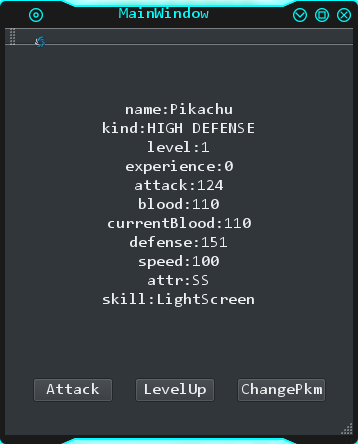
\includegraphics[width=8cm]{stage1-main.png}
\end{figure}
\pagebreak[4]
普通攻击:
\begin{figure}[H]
  \centering
  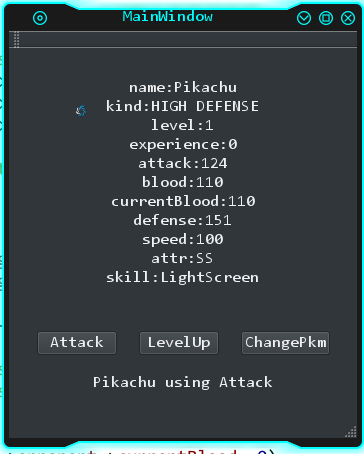
\includegraphics[width=8cm]{stage1-normalAttack.png}
\end{figure}
使用技能:
\begin{figure}[H]
  \centering
  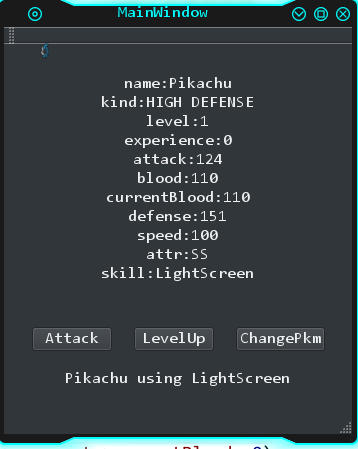
\includegraphics[width=8cm]{stage1-skill.png}
\end{figure}
\pagebreak[4]
升级(升到满级15级后,Level Up按钮将被禁用):
\begin{figure}[H]
  \centering
  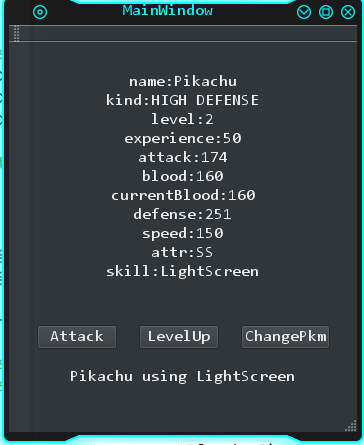
\includegraphics[width=8cm]{stage1-levelUp.png}
\end{figure}
更换小精灵:
\begin{figure}[H]
  \centering
  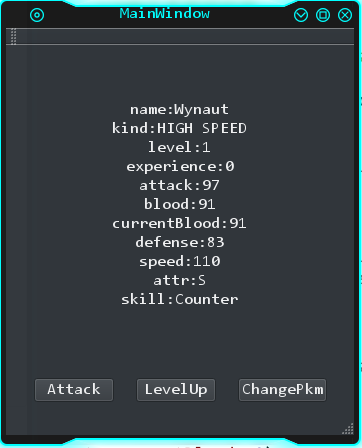
\includegraphics[width=8cm]{stage1-changePkm.png}
\end{figure}
\subsection{第二阶段}
登录界面:
\begin{figure}[H]
  \centering
  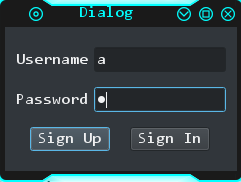
\includegraphics[width=8cm]{stage2-login.png}
\end{figure}
注册:
\begin{figure}[H]
  \centering
  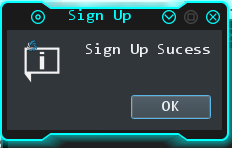
\includegraphics[width=8cm]{stage2-signup.png}
\end{figure}
登录:
\begin{figure}[H]
  \centering
  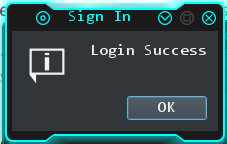
\includegraphics[width=8cm]{stage2-signin.png}
\end{figure}
\pagebreak[4]
主界面:
\begin{figure}[H]
  \centering
  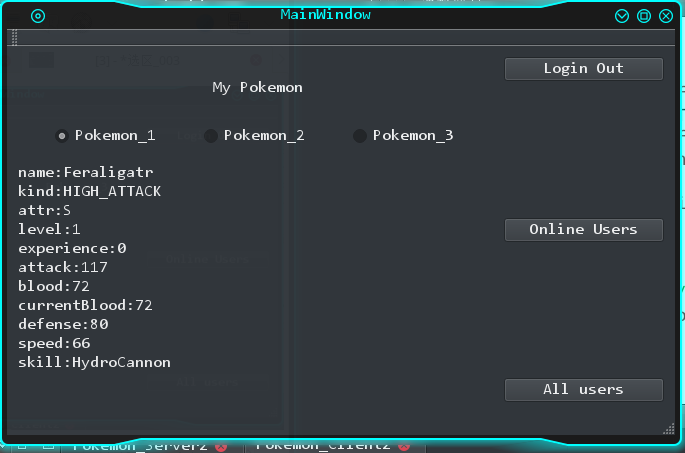
\includegraphics[width=15cm]{stage2-main.png}
\end{figure}
查询在线用户:
\begin{figure}[H]
  \centering
  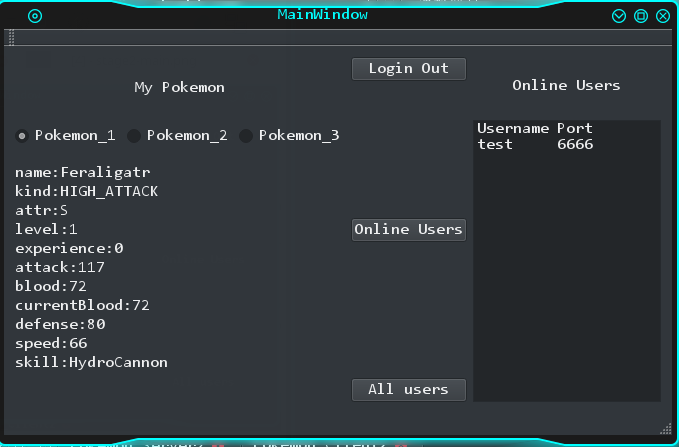
\includegraphics[width=15cm]{stage2-online.png}
\end{figure}
\pagebreak[4]
查询所有用户:
\begin{figure}[H]
  \centering
  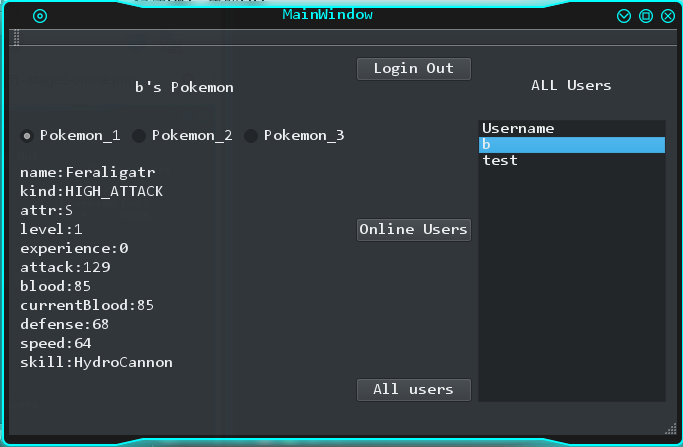
\includegraphics[width=15cm]{stage2-alluser.png}
\end{figure}
\subsection{第三阶段}
登录界面(第二阶段已截取注册界面,故不再截取):
\begin{figure}[H]
  \centering
  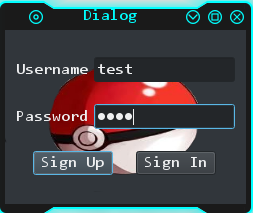
\includegraphics[width=8cm]{stage3-login.png}
\end{figure}
\pagebreak[4]
主界面:
\begin{figure}[H]
  \centering
  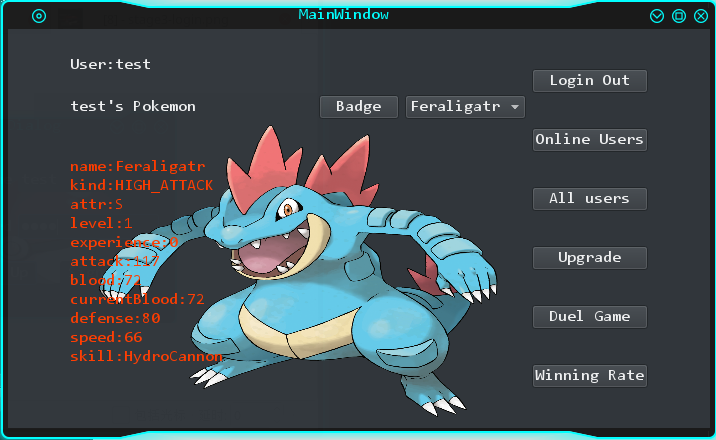
\includegraphics[width=15cm]{stage3-main.png}
\end{figure}
升级赛选择小精灵(决斗赛与此类似,故不再截图):
\begin{figure}[H]
  \centering
  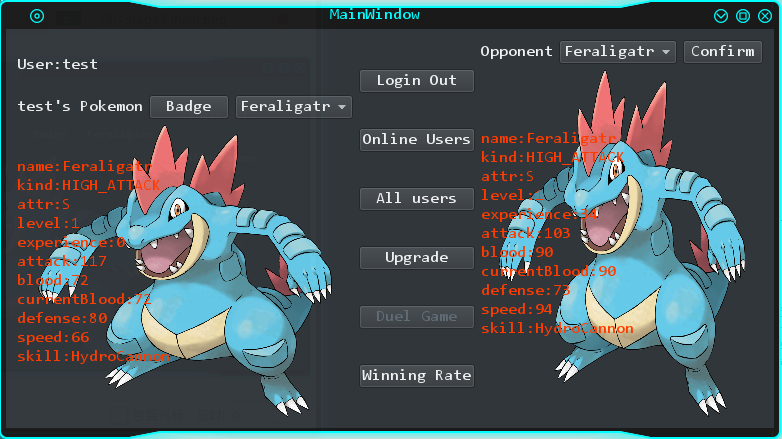
\includegraphics[width=15cm]{stage3-upgrade.png}
\end{figure}
\pagebreak[4]
战斗(左边小精灵使用普通攻击,右边小精灵的攻击则被闪避):
\begin{figure}[H]
  \centering
  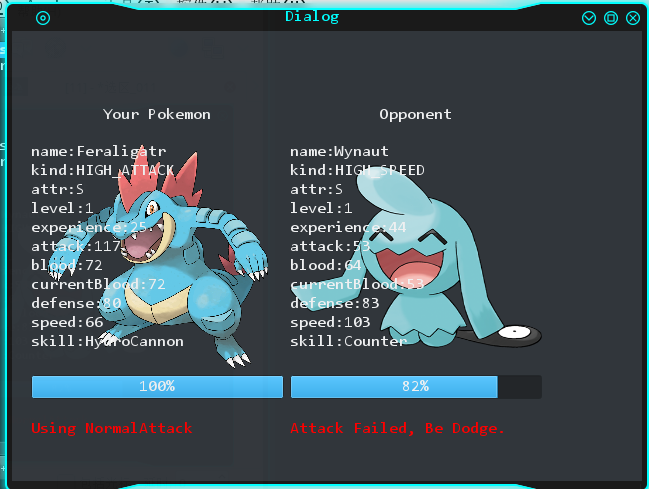
\includegraphics[width=15cm]{stage3-fight.png}
\end{figure}
胜利(从下图可看出小精灵战胜后经验增加,且已升级):
\begin{figure}[H]
  \centering
  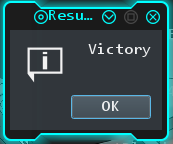
\includegraphics[width=8cm]{stage3-victory.png}
\end{figure}
\pagebreak[4]
决斗赛前(战胜后可获得右边小精灵):
\begin{figure}[H]
  \centering
  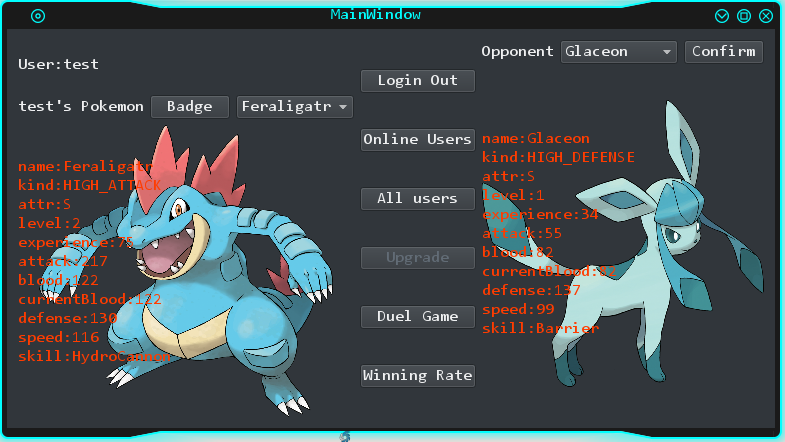
\includegraphics[width=15cm]{stage3-beforeDuel.png}
\end{figure}
决斗赛后(已战胜,且获得右边小精灵):
\begin{figure}[H]
  \centering
  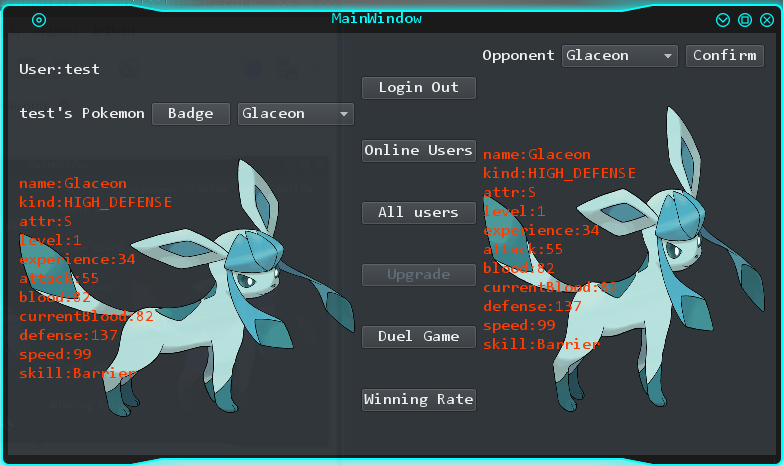
\includegraphics[width=15cm]{stage3-afterDuel.png}
\end{figure}
\pagebreak[4]
战败:
\begin{figure}[H]
  \centering
  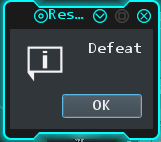
\includegraphics[width=6cm]{stage3-defeat.png}
\end{figure}
战败选择一个小精灵送出:
\begin{figure}[H]
  \centering
  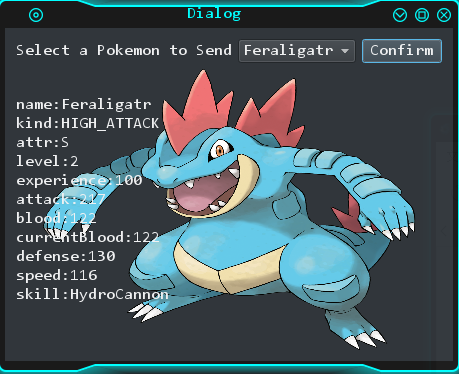
\includegraphics[width=15cm]{stage3-selectPkm.png}
\end{figure}
\pagebreak[4]
查看胜率:
\begin{figure}[H]
  \centering
  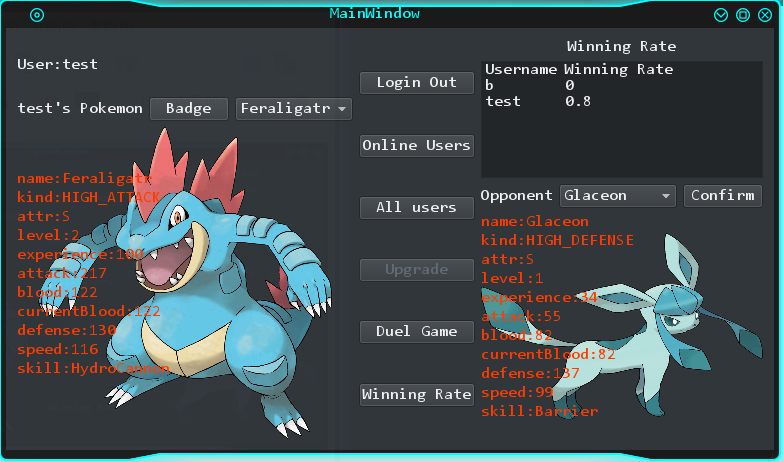
\includegraphics[width=15cm]{stage3-winningRate.png}
\end{figure}
查看徽章:
\begin{figure}[H]
  \centering
  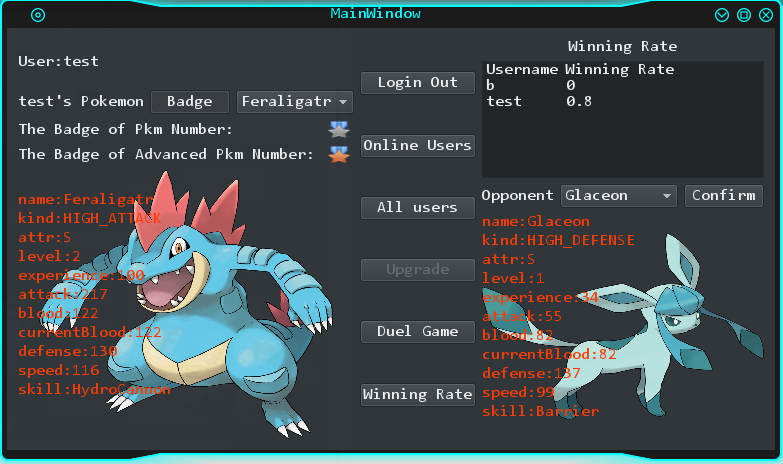
\includegraphics[width=15cm]{stage3-badge.png}
\end{figure}

\section{实验总结}
本次程序设计实践采用C++语言,并综合运用了qt的GUI编程以及socket编程,巩固复习了C++的基础知识,
对类的继承,多态以及封装有了更深刻的认识。此次程序设计使用了socket编程,实际使用了编程来控制网
络传输数据,对网络编程也加深了理解。尤其是网络传输数据时的数据序列化,对网络数据的传输起着至关
重要的作用,可以极大简化数据的封装与读取。此次的C++程序设计实践锻炼了实际编程的能力,把编程知识
实际运用到了现实中,增加了编程的信心。

\end{document}
